% Chapter Template

\chapter{Simulation and Results} % Main chapter title

\label{Chapter4} 

\section{Course generation}.

\begin{figure}[H]
    \centering
    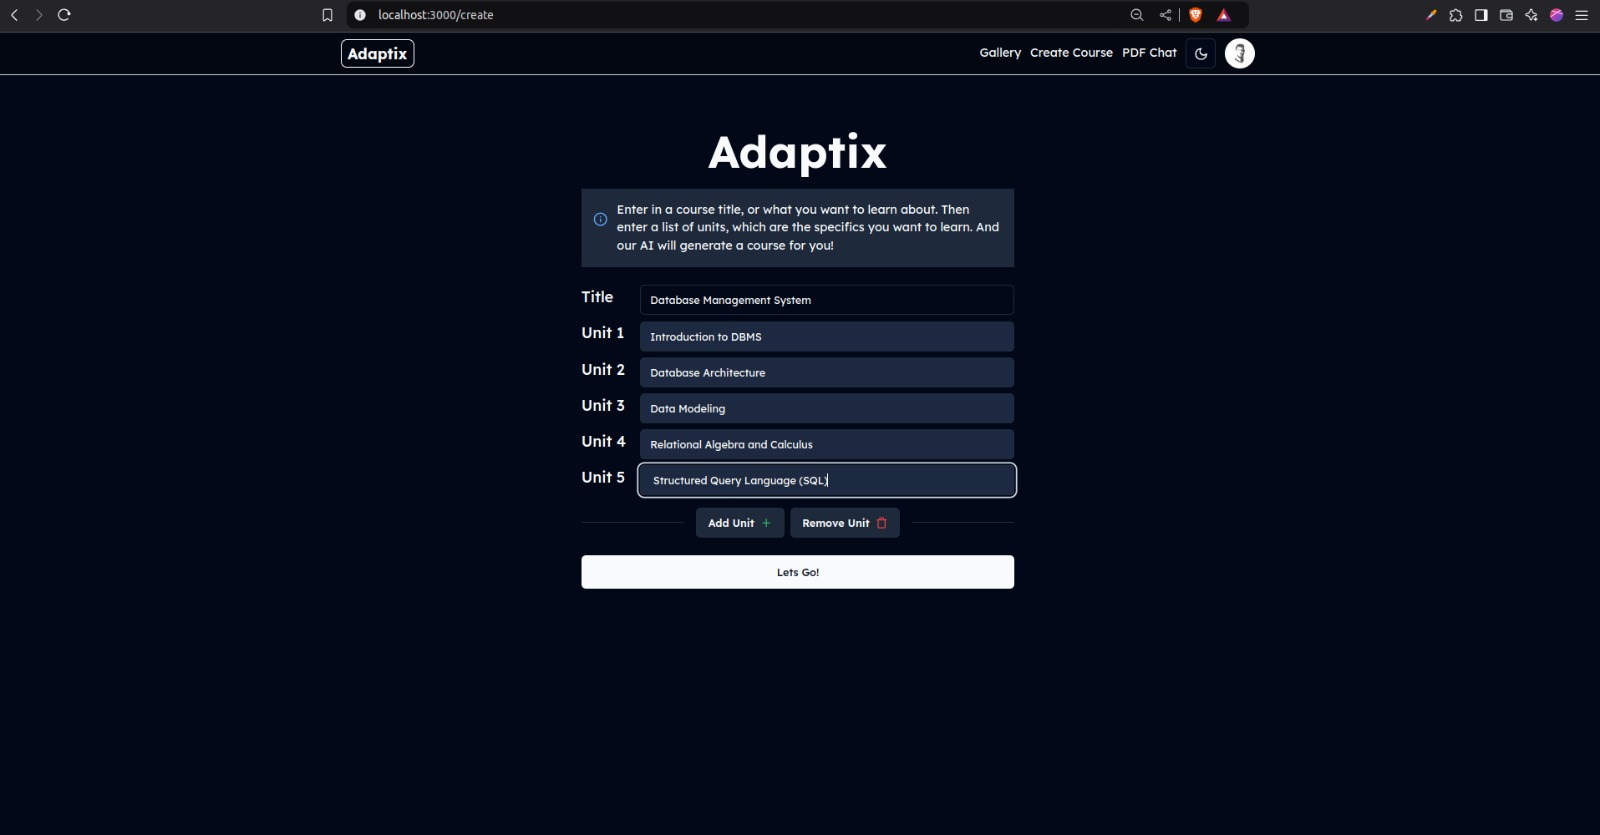
\includegraphics[scale=0.28]{Images/adaptrix-course-gen.jpeg}    
    \caption{Course generation form.}
    \label{fig:course-gen-form}
\end{figure}

The user enters course title and subtopics and clicks on "Let's go".

\section{Generated course and quiz}

\begin{figure}[H]
    \centering
    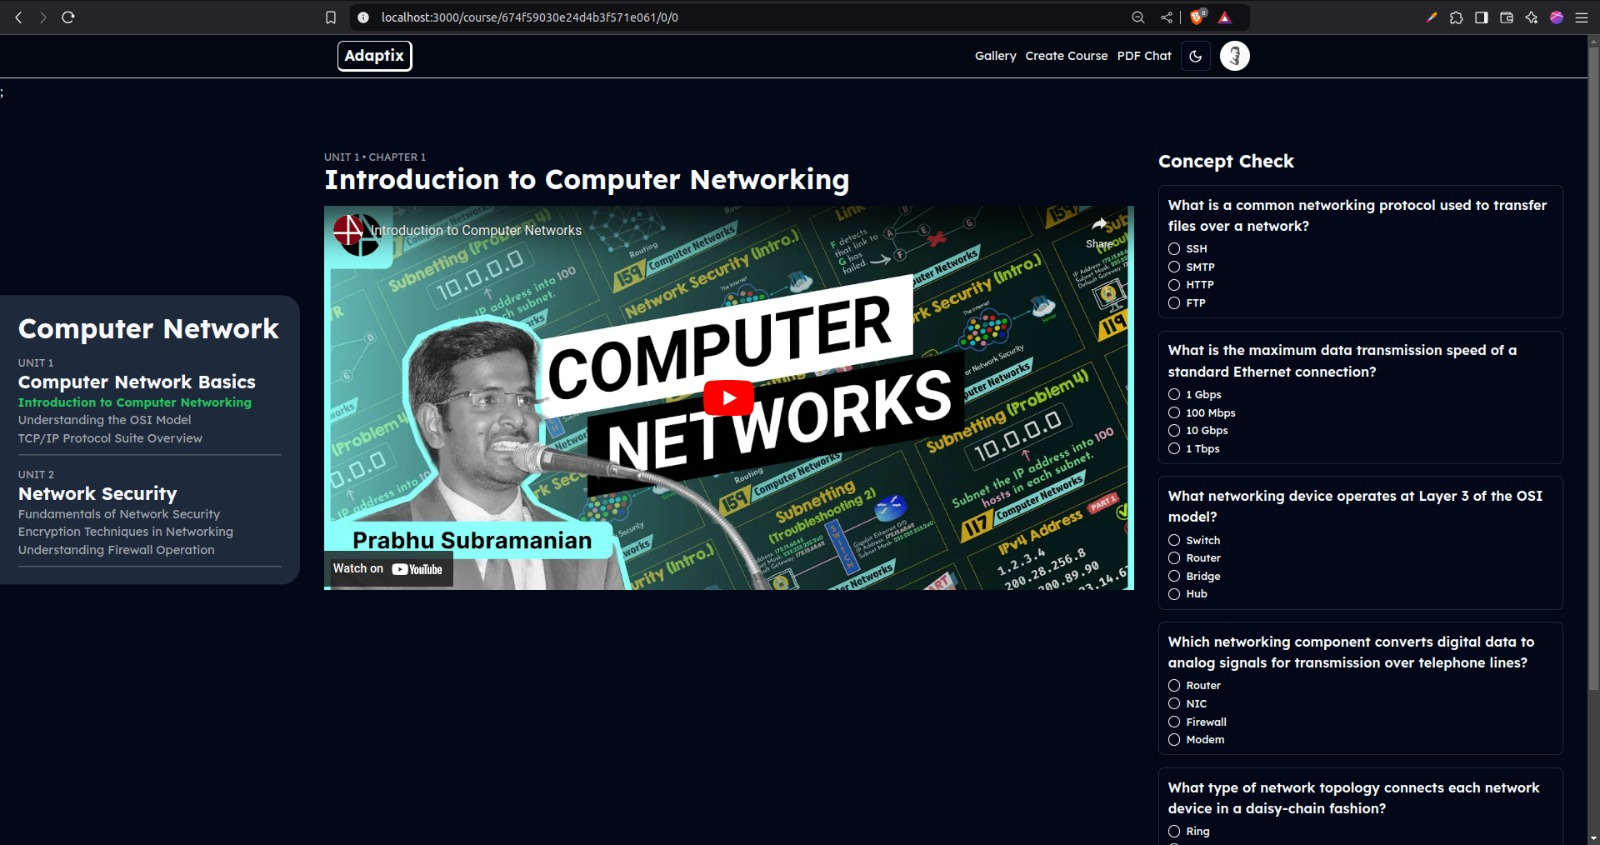
\includegraphics[scale=0.28]{Images/couse-and-quiz.jpeg}
    \caption{Generated course and quiz}
    \label{fig:generated-course}
\end{figure}

A generated course along with concept check quiz is generated based on user input.
\newpage

\section{Chat with PDF}
\begin{figure}[H]
    \centering
    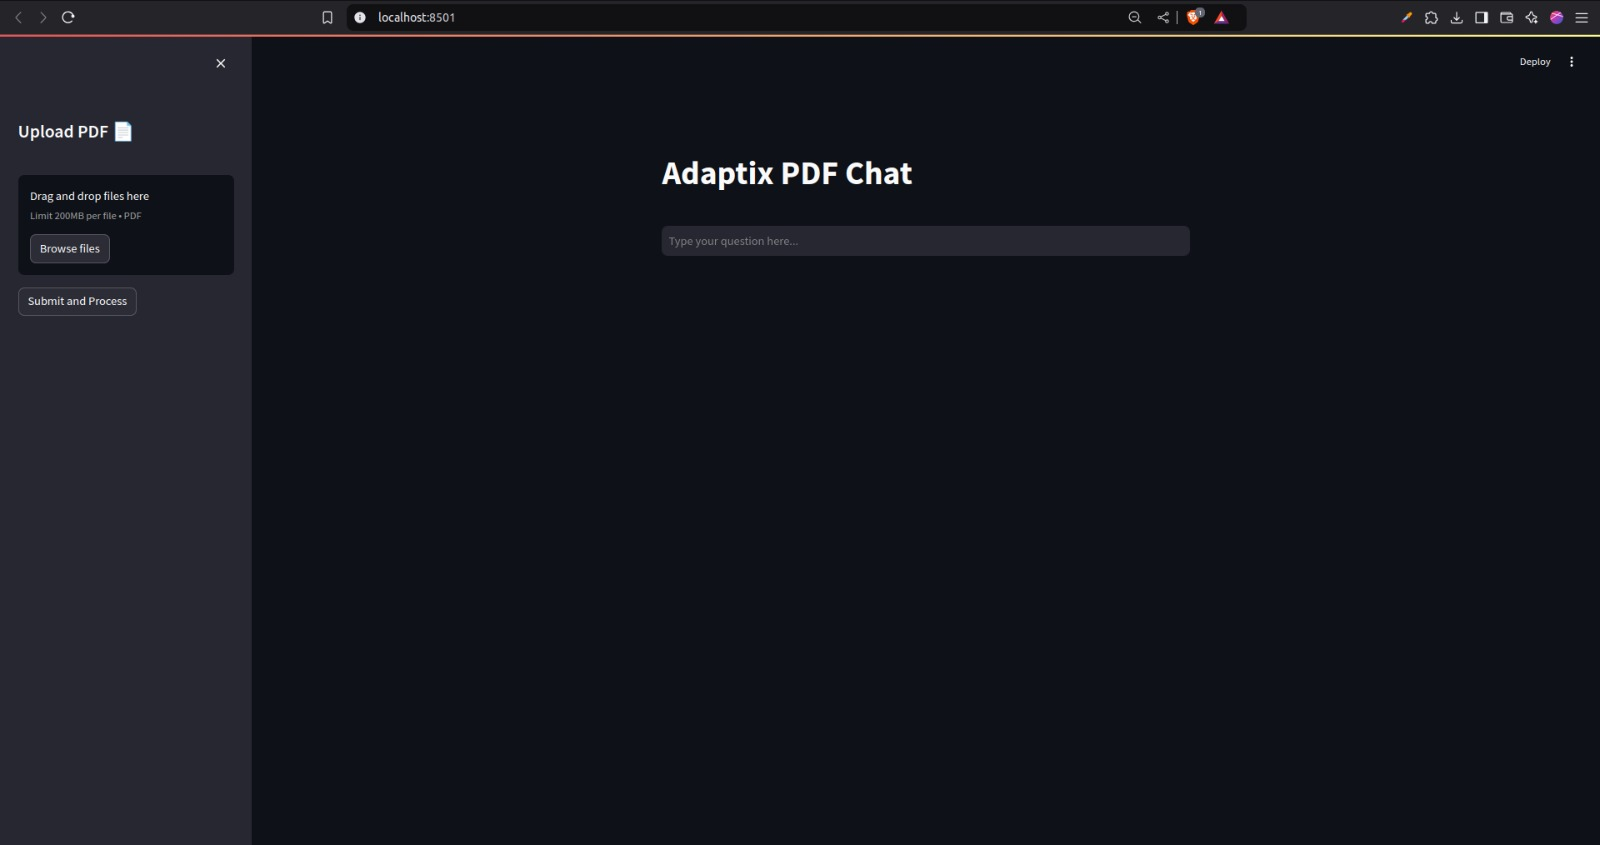
\includegraphics[scale=0.28]{Images/chat-with-pdf.jpeg}
    \caption{A chatbot with context dervied from content in PDF file}
    \label{fig:chat-with-pdf}
\end{figure}

A user can upload a PDF file and then ask questions based on content written in the PDF file.  
This allows easier learning for textual resources.
